\documentclass[tikz]{standalone}
\usepackage{amsmath}
\definecolor{aksen}{HTML}{F7B538}
\definecolor{latar}{HTML}{171D2B}
\definecolor{aksen}{HTML}{F7B538}\definecolor{latar}{HTML}{171D2B}\pagecolor{latar}\begin{document}
\definecolor{aksen}{HTML}{F7B538}\definecolor{latar}{HTML}{171D2B}\pagecolor{latar}\begin{document}
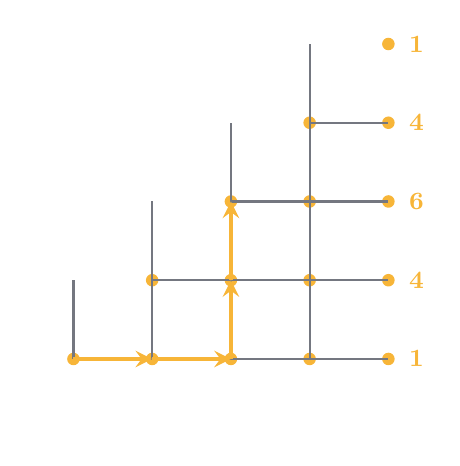
\begin{tikzpicture}[
  scale=1.0,
  dot/.style={circle,fill=aksen,inner sep=1.6pt},
  road/.style={draw=latar!60!white, thick},
  arrow/.style={->, draw=aksen, thick, >=stealth}
]
% grid of intersections 0..4
\foreach \i in {0,...,4}
  \foreach \j in {0,...,\i}
    \node[dot] at (\i,\j) {};
% roads: horizontal and vertical edges of the lattice
\foreach \i in {0,...,3}
  \foreach \j in {0,...,\i} {
    \draw[road] (\i,\j) -- (\i+1,\j);
    \draw[road] (\i,\j) -- (\i,\j+1);
  }
% labels:

\foreach \i/\j/\t in {0/0/1, 1/0/1, 1/1/1, 2/0/1, 2/1/2, 2/2/1, 3/0/1, 3/1/3, 3/2/3, 3/3/1} {
  \node[white, font=\small, anchor=north east, inner sep=1pt] at (\i-0.12,\j-0.12) {\t};
}
\foreach \j/\t in {0/1, 1/4, 2/6, 3/4, 4/1} {
  \node[text=aksen, font=\small\bfseries, anchor=west, inner sep=3pt] at (4.15,\j) {\t};
}

% one example path highlighted: E,E,N,N
\draw[arrow, line width=1.6pt] (0,0) -- (1,0);
\draw[arrow, line width=1.6pt] (1,0) -- (2,0);
\draw[arrow, line width=1.6pt] (2,0) -- (2,1);
\draw[arrow, line width=1.6pt] (2,1) -- (2,2);
\node[white, font=\small] at (1.6,-0.75) {$2+4=6$ jalur lewat titik ini};
\end{tikzpicture}
\end{document}
